\documentclass{article}

\usepackage[italian]{babel}
\usepackage[T1]{fontenc}
\usepackage[utf8]{inputenc}
\usepackage{graphicx}
\usepackage{wrapfig}

\setlength{\parindent}{0pt}

\usepackage{geometry}
\geometry{
	paper=a4paper, % Paper size, change to letterpaper for US letter size
	top=3.25cm, % Top margin
	bottom=4cm, % Bottom margin
	left=3.5cm, % Left margin
	right=3.5cm, % Right margin
	headheight=0.75cm, % Header height
	footskip=1cm, % Space from the bottom margin to the baseline of the footer
	headsep=0.75cm, % Space from the top margin to the baseline of the header
	%showframe, % Uncomment to show how the type block is set on the page
}

\usepackage[semibold]{ebgaramond}
\usepackage{sectsty} % Allows changing the font options for sections in a document

\sectionfont{\fontsize{13.5pt}{18pt}\selectfont} % Set font options for sections
%\subsectionfont{\mdseries\scshape\normalsize} % Set font options for subsections
\subsubsectionfont{\mdseries\upshape\bfseries\normalsize} % Set font options for subsubsections

\usepackage{marginnote} % Required to output text in the margin

\newcommand{\years}[1]{\marginnote{\small #1}} % New command for adding years to the margin
\renewcommand*{\raggedleftmarginnote}{} % Left-align the years in the margin
\setlength{\marginparsep}{-10pt} % Move the margin content closer to the text
\reversemarginpar % Margin text to be output into the left margin instead of the default right margin

\usepackage[usenames, dvipsnames]{xcolor} % Required for specifying colours by name
\usepackage[bookmarks, colorlinks, breaklinks]{hyperref} % Required for links

% Set link colours
\hypersetup{
	linkcolor=blue,
	citecolor=blue,
	filecolor=black,
	urlcolor=MidnightBlue
}

\hypersetup{
	pdftitle={Filippo Barbari - Curriculum vitae},
	pdfauthor={Filippo Barbari}
}

\begin{document}
	
	\begin{wrapfigure}{r}{0.2\textwidth}
		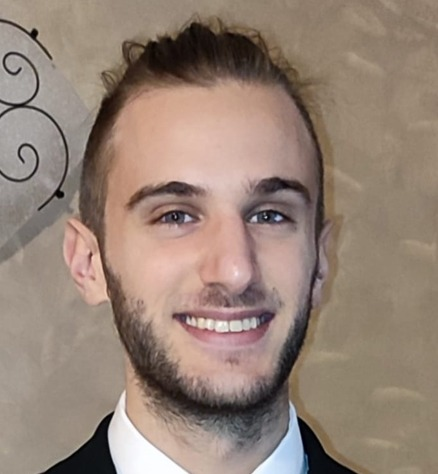
\includegraphics[width=0.18\textwidth]{fototessera}
	\end{wrapfigure}
		
	{\LARGE\bfseries Filippo Barbari} % Name
	\bigskip\bigskip\medskip % Whitespace
	
	Via Emilia 42\\ % Address
	47838 Riccione (RN), Italia
	\medskip % Whitespace
	
	Cellulare: 327-2207037\\
	Fisso: 0541-644233
	\medskip
	
	Email: \href{mailto:filippo.barbari@studio.unibo.it}{filippo.barbari@studio.unibo.it}
	\medskip
	
	Nato: 24 agosto 1999, Rimini (RN), Italia\\ % Date of birth
	Nazionalità: Italiana % Nationality
	
	\section*{Formazione}
	
	\years{2013-2018} Diploma di Maturità conseguito con votazione 90/100 presso Liceo Scientifico A. Volta, Riccione (RN)\\
	\years{2018-2021} Laurea Triennale in Ingegneria e Scienze Informatiche conseguita con votazione 106/110 presso Alma Mater Studiorum Università di Bologna, Campus di Cesena in data 7 ottobre 2021
	
	\subsection*{Esami rilevanti sostenuti durante il corso di laurea}
	
	\begin{tabular}{ll}
		\textbf{Programmazione} & votazione 28/30\\
		\textbf{Algoritmi e Strutture Dati} & votazione 30/30 con lode\\
		\textbf{High-Performance Computing} & votazione 30/30\\
		\textbf{Crittografia} & votazione 30/30
	\end{tabular}
	
	\section*{Lingue}
	
	Italiano: madrelingua\\
	Inglese: FCE livello B-2
	
	% Any final footer text such as a URL to the latest version of this CV, last updated date, compiled in XeTeX, etc
	\begin{center}
		\scriptsize
		Ultimo aggiornamento: \today
	\end{center}
	
\end{document}